%% bare_jrnl.tex
%% V1.4b
%% 2015/08/26
%% by Michael Shell
%% see http://www.michaelshell.org/
%% for current contact information.
%%
%% This is a skeleton file demonstrating the use of IEEEtran.cls
%% (requires IEEEtran.cls version 1.8b or later) with an IEEE
%% journal paper.
%%
%% Support sites:
%% http://www.michaelshell.org/tex/ieeetran/
%% http://www.ctan.org/pkg/ieeetran
%% and
%% http://www.ieee.org/

%%*************************************************************************
%% Legal Notice:
%% This code is offered as-is without any warranty either expressed or
%% implied; without even the implied warranty of MERCHANTABILITY or
%% FITNESS FOR A PARTICULAR PURPOSE! 
%% User assumes all risk.
%% In no event shall the IEEE or any contributor to this code be liable for
%% any damages or losses, including, but not limited to, incidental,
%% consequential, or any other damages, resulting from the use or misuse
%% of any information contained here.
%%
%% All comments are the opinions of their respective authors and are not
%% necessarily endorsed by the IEEE.
%%
%% This work is distributed under the LaTeX Project Public License (LPPL)
%% ( http://www.latex-project.org/ ) version 1.3, and may be freely used,
%% distributed and modified. A copy of the LPPL, version 1.3, is included
%% in the base LaTeX documentation of all distributions of LaTeX released
%% 2003/12/01 or later.
%% Retain all contribution notices and credits.
%% ** Modified files should be clearly indicated as such, including  **
%% ** renaming them and changing author support contact information. **
%%*************************************************************************


% *** Authors should verify (and, if needed, correct) their LaTeX system  ***
% *** with the testflow diagnostic prior to trusting their LaTeX platform ***
% *** with production work. The IEEE's font choices and paper sizes can   ***
% *** trigger bugs that do not appear when using other class files.       ***                          ***
% The testflow support page is at:
% http://www.michaelshell.org/tex/testflow/

\documentclass[journal]{IEEEtran}
%
% If IEEEtran.cls has not been installed into the LaTeX system files,
% manually specify the path to it like:
% \documentclass[journal]{../sty/IEEEtran}





% Some very useful LaTeX packages include:
% (uncomment the ones you want to load)


% *** MISC UTILITY PACKAGES ***
%
%\usepackage{ifpdf}
% Heiko Oberdiek's ifpdf.sty is very useful if you need conditional
% compilation based on whether the output is pdf or dvi.
% usage:
% \ifpdf
%   % pdf code
% \else
%   % dvi code
% \fi
% The latest version of ifpdf.sty can be obtained from:
% http://www.ctan.org/pkg/ifpdf
% Also, note that IEEEtran.cls V1.7 and later provides a builtin
% \ifCLASSINFOpdf conditional that works the same way.
% When switching from latex to pdflatex and vice-versa, the compiler may
% have to be run twice to clear warning/error messages.






% *** CITATION PACKAGES ***
%
%\usepackage{cite}
% cite.sty was written by Donald Arseneau
% V1.6 and later of IEEEtran pre-defines the format of the cite.sty package
% \cite{} output to follow that of the IEEE. Loading the cite package will
% result in citation numbers being automatically sorted and properly
% "compressed/ranged". e.g., [1], [9], [2], [7], [5], [6] without using
% cite.sty will become [1], [2], [5]--[7], [9] using cite.sty. cite.sty's
% \cite will automatically add leading space, if needed. Use cite.sty's
% noadjust option (cite.sty V3.8 and later) if you want to turn this off
% such as if a citation ever needs to be enclosed in parenthesis.
% cite.sty is already installed on most LaTeX systems. Be sure and use
% version 5.0 (2009-03-20) and later if using hyperref.sty.
% The latest version can be obtained at:
% http://www.ctan.org/pkg/cite
% The documentation is contained in the cite.sty file itself.


\usepackage{balance}



% *** GRAPHICS RELATED PACKAGES ***
%
\ifCLASSINFOpdf
   \usepackage[pdftex]{graphicx}
  % declare the path(s) where your graphic files are
  % \graphicspath{{../pdf/}{../jpeg/}}
  % and their extensions so you won't have to specify these with
  % every instance of \includegraphics
   \DeclareGraphicsExtensions{.pdf,.jpeg,.png}
\else
  % or other class option (dvipsone, dvipdf, if not using dvips). graphicx
  % will default to the driver specified in the system graphics.cfg if no
  % driver is specified.
  % \usepackage[dvips]{graphicx}
  % declare the path(s) where your graphic files are
  % \graphicspath{{../eps/}}
  % and their extensions so you won't have to specify these with
  % every instance of \includegraphics
  % \DeclareGraphicsExtensions{.eps}
\fi
% graphicx was written by David Carlisle and Sebastian Rahtz. It is
% required if you want graphics, photos, etc. graphicx.sty is already
% installed on most LaTeX systems. The latest version and documentation
% can be obtained at: 
% http://www.ctan.org/pkg/graphicx
% Another good source of documentation is "Using Imported Graphics in
% LaTeX2e" by Keith Reckdahl which can be found at:
% http://www.ctan.org/pkg/epslatex
%
% latex, and pdflatex in dvi mode, support graphics in encapsulated
% postscript (.eps) format. pdflatex in pdf mode supports graphics
% in .pdf, .jpeg, .png and .mps (metapost) formats. Users should ensure
% that all non-photo figures use a vector format (.eps, .pdf, .mps) and
% not a bitmapped formats (.jpeg, .png). The IEEE frowns on bitmapped formats
% which can result in "jaggedy"/blurry rendering of lines and letters as
% well as large increases in file sizes.
%
% You can find documentation about the pdfTeX application at:
% http://www.tug.org/applications/pdftex




% *** MATH PACKAGES ***
%
\usepackage{mathrsfs,amsmath}
\usepackage{amssymb}
% A popular package from the American Mathematical Society that provides
% many useful and powerful commands for dealing with mathematics.
%
% Note that the amsmath package sets \interdisplaylinepenalty to 10000
% thus preventing page breaks from occurring within multiline equations. Use:
%\interdisplaylinepenalty=2500
% after loading amsmath to restore such page breaks as IEEEtran.cls normally
% does. amsmath.sty is already installed on most LaTeX systems. The latest
% version and documentation can be obtained at:
% http://www.ctan.org/pkg/amsmath





% *** SPECIALIZED LIST PACKAGES ***
%
%\usepackage{algorithmic}
% algorithmic.sty was written by Peter Williams and Rogerio Brito.
% This package provides an algorithmic environment fo describing algorithms.
% You can use the algorithmic environment in-text or within a figure
% environment to provide for a floating algorithm. Do NOT use the algorithm
% floating environment provided by algorithm.sty (by the same authors) or
% algorithm2e.sty (by Christophe Fiorio) as the IEEE does not use dedicated
% algorithm float types and packages that provide these will not provide
% correct IEEE style captions. The latest version and documentation of
% algorithmic.sty can be obtained at:
% http://www.ctan.org/pkg/algorithms
% Also of interest may be the (relatively newer and more customizable)
% algorithmicx.sty package by Szasz Janos:
% http://www.ctan.org/pkg/algorithmicx




% *** ALIGNMENT PACKAGES ***
%
%\usepackage{array}
% Frank Mittelbach's and David Carlisle's array.sty patches and improves
% the standard LaTeX2e array and tabular environments to provide better
% appearance and additional user controls. As the default LaTeX2e table
% generation code is lacking to the point of almost being broken with
% respect to the quality of the end results, all users are strongly
% advised to use an enhanced (at the very least that provided by array.sty)
% set of table tools. array.sty is already installed on most systems. The
% latest version and documentation can be obtained at:
% http://www.ctan.org/pkg/array


% IEEEtran contains the IEEEeqnarray family of commands that can be used to
% generate multiline equations as well as matrices, tables, etc., of high
% quality.




% *** SUBFIGURE PACKAGES ***
%\ifCLASSOPTIONcompsoc
%  \usepackage[caption=false,font=normalsize,labelfont=sf,textfont=sf]{subfig}
%\else
%  \usepackage[caption=false,font=footnotesize]{subfig}
%\fi
% subfig.sty, written by Steven Douglas Cochran, is the modern replacement
% for subfigure.sty, the latter of which is no longer maintained and is
% incompatible with some LaTeX packages including fixltx2e. However,
% subfig.sty requires and automatically loads Axel Sommerfeldt's caption.sty
% which will override IEEEtran.cls' handling of captions and this will result
% in non-IEEE style figure/table captions. To prevent this problem, be sure
% and invoke subfig.sty's "caption=false" package option (available since
% subfig.sty version 1.3, 2005/06/28) as this is will preserve IEEEtran.cls
% handling of captions.
% Note that the Computer Society format requires a larger sans serif font
% than the serif footnote size font used in traditional IEEE formatting
% and thus the need to invoke different subfig.sty package options depending
% on whether compsoc mode has been enabled.
%
% The latest version and documentation of subfig.sty can be obtained at:
% http://www.ctan.org/pkg/subfig




% *** FLOAT PACKAGES ***
%
%\usepackage{fixltx2e}
% fixltx2e, the successor to the earlier fix2col.sty, was written by
% Frank Mittelbach and David Carlisle. This package corrects a few problems
% in the LaTeX2e kernel, the most notable of which is that in current
% LaTeX2e releases, the ordering of single and double column floats is not
% guaranteed to be preserved. Thus, an unpatched LaTeX2e can allow a
% single column figure to be placed prior to an earlier double column
% figure.
% Be aware that LaTeX2e kernels dated 2015 and later have fixltx2e.sty's
% corrections already built into the system in which case a warning will
% be issued if an attempt is made to load fixltx2e.sty as it is no longer
% needed.
% The latest version and documentation can be found at:
% http://www.ctan.org/pkg/fixltx2e


%\usepackage{stfloats}
% stfloats.sty was written by Sigitas Tolusis. This package gives LaTeX2e
% the ability to do double column floats at the bottom of the page as well
% as the top. (e.g., "\begin{figure*}[!b]" is not normally possible in
% LaTeX2e). It also provides a command:
%\fnbelowfloat
% to enable the placement of footnotes below bottom floats (the standard
% LaTeX2e kernel puts them above bottom floats). This is an invasive package
% which rewrites many portions of the LaTeX2e float routines. It may not work
% with other packages that modify the LaTeX2e float routines. The latest
% version and documentation can be obtained at:
% http://www.ctan.org/pkg/stfloats
% Do not use the stfloats baselinefloat ability as the IEEE does not allow
% \baselineskip to stretch. Authors submitting work to the IEEE should note
% that the IEEE rarely uses double column equations and that authors should try
% to avoid such use. Do not be tempted to use the cuted.sty or midfloat.sty
% packages (also by Sigitas Tolusis) as the IEEE does not format its papers in
% such ways.
% Do not attempt to use stfloats with fixltx2e as they are incompatible.
% Instead, use Morten Hogholm'a dblfloatfix which combines the features
% of both fixltx2e and stfloats:
%
% \usepackage{dblfloatfix}
% The latest version can be found at:
% http://www.ctan.org/pkg/dblfloatfix




%\ifCLASSOPTIONcaptionsoff
%  \usepackage[nomarkers]{endfloat}
% \let\MYoriglatexcaption\caption
% \renewcommand{\caption}[2][\relax]{\MYoriglatexcaption[#2]{#2}}
%\fi
% endfloat.sty was written by James Darrell McCauley, Jeff Goldberg and 
% Axel Sommerfeldt. This package may be useful when used in conjunction with 
% IEEEtran.cls'  captionsoff option. Some IEEE journals/societies require that
% submissions have lists of figures/tables at the end of the paper and that
% figures/tables without any captions are placed on a page by themselves at
% the end of the document. If needed, the draftcls IEEEtran class option or
% \CLASSINPUTbaselinestretch interface can be used to increase the line
% spacing as well. Be sure and use the nomarkers option of endfloat to
% prevent endfloat from "marking" where the figures would have been placed
% in the text. The two hack lines of code above are a slight modification of
% that suggested by in the endfloat docs (section 8.4.1) to ensure that
% the full captions always appear in the list of figures/tables - even if
% the user used the short optional argument of \caption[]{}.
% IEEE papers do not typically make use of \caption[]'s optional argument,
% so this should not be an issue. A similar trick can be used to disable
% captions of packages such as subfig.sty that lack options to turn off
% the subcaptions:
% For subfig.sty:
% \let\MYorigsubfloat\subfloat
% \renewcommand{\subfloat}[2][\relax]{\MYorigsubfloat[]{#2}}
% However, the above trick will not work if both optional arguments of
% the \subfloat command are used. Furthermore, there needs to be a
% description of each subfigure *somewhere* and endfloat does not add
% subfigure captions to its list of figures. Thus, the best approach is to
% avoid the use of subfigure captions (many IEEE journals avoid them anyway)
% and instead reference/explain all the subfigures within the main caption.
% The latest version of endfloat.sty and its documentation can obtained at:
% http://www.ctan.org/pkg/endfloat
%
% The IEEEtran \ifCLASSOPTIONcaptionsoff conditional can also be used
% later in the document, say, to conditionally put the References on a 
% page by themselves.




% *** PDF, URL AND HYPERLINK PACKAGES ***
%
%\usepackage{url}
% url.sty was written by Donald Arseneau. It provides better support for
% handling and breaking URLs. url.sty is already installed on most LaTeX
% systems. The latest version and documentation can be obtained at:
% http://www.ctan.org/pkg/url
% Basically, \url{my_url_here}.




% *** Do not adjust lengths that control margins, column widths, etc. ***
% *** Do not use packages that alter fonts (such as pslatex).         ***
% There should be no need to do such things with IEEEtran.cls V1.6 and later.
% (Unless specifically asked to do so by the journal or conference you plan
% to submit to, of course. )


% correct bad hyphenation here
\hyphenation{op-tical net-works semi-conduc-tor}


\begin{document}
%
% paper title
% Titles are generally capitalized except for words such as a, an, and, as,
% at, but, by, for, in, nor, of, on, or, the, to and up, which are usually
% not capitalized unless they are the first or last word of the title.
% Linebreaks \\ can be used within to get better formatting as desired.
% Do not put math or special symbols in the title.
\title{Graph Optimization Approach to Localization \\ with IMU and Ultra-Wideband Measurements}
%
%
% author names and IEEE memberships
% note positions of commas and nonbreaking spaces ( ~ ) LaTeX will not break
% a structure at a ~ so this keeps an author's name from being broken across
% two lines.
% use \thanks{} to gain access to the first footnote area
% a separate \thanks must be used for each paragraph as LaTeX2e's \thanks
% was not built to handle multiple paragraphs
%

\author{Chen Wang\IEEEauthorrefmark{2},
        \IEEEauthorrefmark{1}Xu Fang\IEEEauthorrefmark{2},
        Thien-Minh Nguyen, 
        Lihua
        Xie~\IEEEmembership{Fellow,~IEEE}% <-this % stops a space
\thanks{The authors are with School of Electrical and Electronic Engineering, Nanyang Technological University, Singapore (e-mail: wang.chen@zoho.com, \IEEEauthorrefmark{1}fa0001xu@e.ntu.edu.sg, e150040@e.ntu.edu.sg, elhxie@ntu.edu.sg) .}% <-this % stops a space
\thanks{\IEEEauthorrefmark{2}Chen Wang and Xu Fang are joint first authors.}% <-this % stops a space
}

% note the % following the last \IEEEmembership and also \thanks - 
% these prevent an unwanted space from occurring between the last author name
% and the end of the author line. i.e., if you had this:
% 
% \author{....lastname \thanks{...} \thanks{...} }
%                     ^------------^------------^----Do not want these spaces!
%
% a space would be appended to the last name and could cause every name on that
% line to be shifted left slightly. This is one of those "LaTeX things". For
% instance, "\textbf{A} \textbf{B}" will typeset as "A B" not "AB". To get
% "AB" then you have to do: "\textbf{A}\textbf{B}"
% \thanks is no different in this regard, so shield the last } of each \thanks
% that ends a line with a % and do not let a space in before the next \thanks.
% Spaces after \IEEEmembership other than the last one are OK (and needed) as
% you are supposed to have spaces between the names. For what it is worth,
% this is a minor point as most people would not even notice if the said evil
% space somehow managed to creep in.



% The paper headers
\markboth{Journal of \LaTeX\ Class Files,~Vol.~14, No.~8, August~2015}%
{Shell \MakeLowercase{\textit{et al.}}: Bare Demo of IEEEtran.cls for IEEE Journals}
% The only time the second header will appear is for the odd numbered pages
% after the title page when using the twoside option.
% 
% *** Note that you probably will NOT want to include the author's ***
% *** name in the headers of peer review papers.                   ***
% You can use \ifCLASSOPTIONpeerreview for conditional compilation here if
% you desire.




% If you want to put a publisher's ID mark on the page you can do it like
% this:
%\IEEEpubid{0000--0000/00\$00.00~\copyright~2015 IEEE}
% Remember, if you use this you must call \IEEEpubidadjcol in the second
% column for its text to clear the IEEEpubid mark.



% use for special paper notices
%\IEEEspecialpapernotice{(Invited Paper)}




% make the title area
\maketitle

% As a general rule, do not put math, special symbols or citations
% in the abstract or keywords.
\begin{abstract}
An ultra-wideband (UWB) aided localization system is presented.
Existing filter-based methods using UWB need  kinetic model which is generally hard to obtain because of the complex structure of robots. This paper proposes a graph optimization approach to localization with inertial measurement unit (IMU) and UWB measurements which converts the localization problem into an optimization problem on Lie-Manifold, so that  kinetic model can be avoided. This method makes full use of measurement data to localize a robot with acceptable computational complexity.
It is achieved by minimizing the trajectory error based on several constrained equations arising from different types of sensor measurements. Our first contribution is graph realization in Manifold instead of Euclidean space for  UWB-based systems, and new type of edge is defined and created in order to apply exiting graph optimization tool. Our second contribution is online approach that enables this approach to robots with ultra-low power processor.
Experiments under a variety of scenarios verify the stability of this method and demonstrate that the algorithm achieves a much higher localization accuracy  than the filter-based methods.
\end{abstract}

% Note that keywords are not normally used for peerreview papers.
\begin{IEEEkeywords}
Ultra-Wideband (UWB), Inertial Measurement Unit (IMU), Localization, Lie-Manifold,  Unmanned Aerial Vehicle (UAV).
\end{IEEEkeywords}


% For peer review papers, you can put extra information on the cover
% page as needed:
% \ifCLASSOPTIONpeerreview
% \begin{center} \bfseries EDICS Category: 3-BBND \end{center}
% \fi
%
% For peerreview papers, this IEEEtran command inserts a page break and
% creates the second title. It will be ignored for other modes.
\IEEEpeerreviewmaketitle



\section{Introduction}
% The very first letter is a 2 line initial drop letter followed
% by the rest of the first word in caps.
% 
% form to use if the first word consists of a single letter:
% \IEEEPARstart{A}{demo} file is ....
% 
% form to use if you need the single drop letter followed by
% normal text (unknown if ever used by the IEEE):
% \IEEEPARstart{A}{}demo file is ....
% 
% Some journals put the first two words in caps:
% \IEEEPARstart{T}{his demo} file is ....
% 
% Here we have the typical use of a "T" for an initial drop letter
% and "HIS" in caps to complete the first word.
\IEEEPARstart{l}{ocalization} accuracy and speed play an important role in robot-related applications, such as path following, target searching and obstacle avoidance. The success of such applications relies on the localization algorithm and performance of localization-related sensors. However, some existing localization technologies are difficult or expensive to be deployed directly. For example, the widely-used Global Positioning System (GPS) can only be applied in outdoor environment due to the non-line of sight (NLOS) blockage in indoor environment. The vision-based real-time simultaneous localization and mapping (SLAM)  technologies  \cite{Engel:2014fd, JakobEngel:2014uc, AnkurHanda:2014ub} have an unacceptable drift without odometer correction and need significant computational resources for dense mapping, which are not suitable for ultra-low power processor. The WiFi-based localization \cite{Chen:2015bk,Sen:2013tv,Deng:2015js} has the problem of large  fluctuations caused by the variation of signals and its unsatisfactory accuracy makes it inapplicable to robots such as unmanned aerial vehicle (UAV). Motion capture systems can provide millimeter level of accuracy and focus on challenging tasks such as formation and swarming \cite{Lupashin:2014bf,Kushleyev:2013wy}. But they are very expensive and only applicable to small-scale spaces. 
An alternative method which utilizes the ultra-wideband communication has attracted researchers' attention due to  its robustness to multipath and non-line of sight effects. This characteristic brings about high speed communication and  ranging measurement. Robot carrying a UWB module is able to calculate its relative distances to other UWB modules (referred to as anchors) by measuring the time of arrival (TOA), which is then used for estimating its own position. The existing results using UWB for localization can be found in \cite{Ledergerber:2015ur,J:2008wy,Alsindi:2009ig,Guo:2016ff,Dardari:2009dd}. For UWB-based localization, the robots \cite{Mueller:2015gm} are able to locate themselves by using a set of fixed anchors, and an extended aerodynamic model for localization under the assumption of no wind. The specification of a time of flight-based ranging protocol \cite{Dalce:2013gc} is proposed for localization without involving a localization server. Cooperative UWB localization tackling the trade-off between accuracy and delay is considered in \cite{Garcia:2014gt}, which derives lower bounds on UWB positioning accuracy. For localization-related applications, the localization is applied to swarms of robots in \cite{Prorok:2014jc}, which utilizes tessellated maps that associate probabilistic error models for localization.  The capability of supporting multi-UAV formation is presented in \cite{Anonymous:tWWRLPVI}. But this localization system needs to be fused with other sensors to obtain altitude estimation. Without fixed-anchors, a small number of anchors mounted on the moving robots can be used for target tracking\cite{Hepp:2016hq}, which only require that the target be equipped with a UWB tranceiver. One potential application of UWB is the relative localization for moving robots in GPS-denied environments, which is the key technology for applications such as relative position information based formation and swarming algorithms. To improve the accuracy of UWB-based localization, some papers focus on the problem of optimal sensor placement \cite{Bishop:2010kv, Martinez:2006ff, Isaacs:2009ub}. The common conclusion is that the anchors should be spread evenly about the robot.

The current UWB-based localization methods are mainly based on Kalman filters such as Extended Kalman Filter (EKF) and Unscented Kalman Filter (UKF) \cite{Benini:2012br, Anonymous:5gCbn1Jl,UmaMageswari:2012vd}. The EKF can provide real-time vehicle position updates which relies on linear dynamic models. UKF is an improvement over EKF. Deterministic sampling approach is used to pick a minimal set of sample points (sigma points) around the mean. These sigma points are then propagated through the non-linear model, from which a new mean and covariance estimates are formed and a better estimation of the state can be obtained based on these propagated sigma points. Other methods are Particle filters and Non-linear regression \cite{Anonymous:tWWRLPVI,Rai:2012tv,Youssef:2005tz}. Particle filters uses a genetic mutation-selection sampling approach for estimation, with a set of particles to represent the posterior distribution of stochastic process. Non-linear regression is a form of regression analysis which models observational data by a function. 

The common characteristic of these methods is that they need kinetic model. However, an obvious problem is that kinetic model is always nonlinear and also hard to obtain due to the complex structure of robots. The simplified or linearized kinetic model will bring unpredictable localization error. Also, these methods only utilize current measurement and a priori estimate for each estimation, which will diverge if the signal is lost for short time.  

Considering above drawbacks, a localization method is presented in this paper to improve the accuracy and stability of UWB-based localization. Inspired by the theory of Lie group and Lie algebra, the robot or anchor poses at each time instant can be regarded as a rigid transformation in 3-D space, resulting in several constrained equations. Therefore, the task of localization becomes an optimization problem on Lie-Manifolds with various constraints due to different kinds of measurements. A remarkable advantage of the proposed method is that the kinetic model of the robot is avoided and the position of the robot can be estimated by calculating the optimal solution to the optimization problem. It is worth noting that at each time instant the newly added transformations and constrained equations are able to correct the previous estimate of position. The proposed method is robust to short lost in signal because it utilizes not only current measurements but also previous measurements to avoid divergence. This characteristic adds more constraints to estimation, which will improve the estimation accuracy.

\section{Related Work}
\label{work}

The literature review only focuses on localization technologies that are most closely related to our work.

\subsection{Simultaneous Localization and Mapping}

The similar technology for Lie-Manifolds-based localization is used in SLAM technology \cite{Forster:U0j63nKN, Endres:2014ib,Engel:2017cg}, which not only builds constrained equations between adjacent frames, but also between landmarks and frames.  The landmarks in SLAM serve as similar function as anchors in UWB-based localization. These constrained equations among frames and landmarks mainly describe their pose relationships. 

For camera-based system, iterative closest point is one of the most widely used algorithms which need powerful GPU to process pose relationships. Feature-based \cite{Whelan:2017fn, Newcombe:2015us} and direct methods \cite{Forster:2014ts, MurArtal:2015iua} use iterative methods such as Gauss-Newton to match the images for monocular, stereo cameras and depth cameras. The deep learning based SLAM \cite{Tateno:2017tv, DeTone:2017wk} also need iterative solutions to adjust the weights in neural networks. A non-iterative SLAM is presented in \cite{Wang:2017tx} to reduce the computational requirements dramatically, which demonstrates a new objective function with closed-form solution. The rotational motions are decoupled from transnational motions. The transnational motion model can be obtained by single key-frame training. Then robot motions are obtained by recoupling the estimation in rotational and translational spaces. 

Compared with UWB-based localization, camera-based systems have long range and high resolution, but \cite{Aulinas:2008wj} the computation cost is considerably high so that it can not be applied to robots with ultra-low power processor. In addition, the good visual features are difficult to extract and match, and SLAM has an unacceptable drift without loop closure detection. Other SLAM systems such as laser-based and sonar-based systems depend on inertial sensors. The small errors in inertial sensors can lead to large localization errors. 

It is well-known that graph optimization approaches are superior to filtering approaches in terms of robustness. We propose to apply this technique to the problem of localization using UWB-IMU data fusion. The relationships of frames and landmarks in SLAM are pose constraints. But the relationships in UWB-based systems include distance relationship between robot and anchors, which is a challenge for applying existing graph optimization tool to UWB-based systems because it doesn't include this type of relationship in the existing open-source optimization libraries. The new functions need to be defined and created in order to apply existing graph optimization tool to UWB-based systems. This paper aims to combine the advantages of graph optimization method and good performance of UWB sensor, and propose a novel localization structure for UWB-based localization which not only has less computation cost than that in SLAM but also has better localization accuracy than existing UWB-based localization methods.


\subsection{Graph Realization}

The literature on graph realization problem focuses on finding Euclidean positions for the vertices of a graph given a set of edge lengths, which is different from SLAM. A theory of network localization in terms of graph rigidity theory is proposed \cite{Aspnes:2006up} to find a unique realization. However, alternative incorrect realizations may arise under the presence of measurement noise. \cite{XingboWang:2012kw} proposes a noise model to get the noise characteristics of UWB measurements. Then uses a maximum likelihood estimator for  prelocalization in Cartesian coordinates and obtaining noise covariance matrix that is used in Kalman filter to update the state estimation recursively.  \cite{DiFranco:2017ib} proposes a method for calibration-free, infrastructure-free localization in sensor networks. The generalization of classical multidimensional scaling algorithm is proposed to account for measurements and this method circumvents a-priori calibration. Similarly, several works addresses the geometric relations between robots and anchors \cite{Diao:2014uh, Khan:2009ui}. 

Compared with these UWB-based graph realizations, our approach exploits graph realization in Manifold instead of Euclidean space. The poses instead of translations of robot are used to build constrained equations directly between robot and anchors. The graph realization in Manifold
brings better localization accuracy than that in Euclidean space because graph optimization approaches are superior to filtering approaches in terms of robustness.

UWB localization may be trapped in NLOS scenarios that induce multi-path signal components. The methods for this problem can be categorized into two groups: those that only use LOS measurements \cite{Chan:2006id,LiCong:2005jf}, and those that use both NLOS and LOS measurements \cite{Anonymous:juzQYOCo, Venkatraman:2004gc}. Our approach is to design an outlier rejector that rejects the NLOS measurements and only uses LOS measurements for localization.

\subsection{Contributions}
In contrast to existing UWB-based localization methods, the novelty of our approach is summarized as follows: $(\romannumeral1)$ we do not need kinetic model for UWB-based localization, which is different with filtering-based localization methods, $(\romannumeral2)$ we exploit graph realization in Manifold instead of Euclidean space and new type of edge (distance edge) is defined and created in order to apply existing graph optimization tool to UWB-based systems,$(\romannumeral3)$ A flexible moving window is designed to decrease the computation, which enables this approach to robots with ultra-low power processor, $(\romannumeral4)$ Smooth edge between adjacent robot poses and its covariance matrices are defined and designed to improve the possibility of converging to optimal solutions.
 The existing algorithms have incompatible accuracy in altitude without adding other sensors such as Lidar sensor for estimating altitude , which is a persist issue. The reason for this phenomenon is shown by Fig. \ref{fig1}. The robot is at position $A$, but the estimation is at position $B$ which is a sub-optimal solution because it has the approximate distances away from four anchors as at position $A$. This phenomenon will cause big estimation error along the altitude $z$. One possible way to solve this problem is to add more anchors or place one anchor on the ceiling. But for outdoor environment, it is difficult to place anchor on the ceiling. 

\begin{figure}[!t]
 \centering
\includegraphics[width=0.9\linewidth]{pic/sub-optimal.pdf}
\caption{The robot is at position $A$, but the estimation is at position $B$ which has the same distances away from four anchors as at position $A$.}
\label{fig1}
\end{figure}

An remarkable advantage of our approach is that the accuracy in altitude enables UWB-based localization to 3D space application in outdoor environment. The simplified or linearized kinetic model will bring unpredictable localization error. Compared with existing UWB-based localization methods that only utilize current measurement and a priori estimate for each estimation based on simplified or linearized kinetic model, our approach do not need kinetic model and utilizes not only current measurements but also previous measurements to avoid divergence. This character adds more constraints to estimation, which brings better estimation accuracy in altitude under the same conditions.
The main contributions of this paper are: 
\begin{enumerate}
\item An novel online algorithm for UWB-based localization. The UWB and IMU sensor measurements are fused for graph realization, which is different from existing UWB-IMU data fusion using filter-based localization;
\item A framework for UWB-based localization using Lie Manifold optimization method. This framework is not only suitable for UWB and IMU based localization, but also can be extended to applications with other sensors such as WiFi and optical flow sensors;
\item The design of outlier rejector.  Outlier rejector is proposed for rejecting NLOS measurements, which enables this approach to NLOS environment.
\item The design of flexible moving window. The flexible moving window decreases the computation and uses previous and newly measurements for localization. The proposed method is robust to short lost in signal because it uses previous and current measurements for localization instead of only using a priori estimate and current measurement in filtering-based methods. Moreover, at each time instant the newly added transformations and constrained equations are able to correct the previous estimate of position.
\item The implementation of the UWB-based localization method for unmanned aerial vehicles. Sensor data are integrated into a ROS-based robotic localization system. The experiment results verify the higher localization accuracy compared with traditional localization methods, especially in altitude. 
\end{enumerate}

It is worth noting that this technology is being commercialized because of its advantage in  localization accuracy without adding other sensors such as Lidar sensor for estimating altitude. An technological company in Singapore is using this technique for aircraft inspection.

% This paper is organized as follows: Section \ref{sec:preliminary} provides a summary of relevant mathematical preliminaries for localization. In Section \ref{a4}, three kinds of measurement functions used for constructing constrained equations are defined, and the problem of localization with IMU and UWB sensors is formulated. In Section \ref{a6}, an optimization algorithm is presented on Lie-Manifold. Section \ref{a5} shows the advantages of our method compared with existing localization methods. Section \ref{a7} and \ref{a8} provide the details of experiments for localization. Section \ref{a9} ends this paper with conclusions.


\begin{figure*}[!t]
\centering
\includegraphics[width=0.7\linewidth]{pic/uwb.pdf}
\caption{Localization system used for constructing constrained equations are shown in this figure. Two robots move in 3-D space and four anchors are placed in fixed position. Each robot is equipped with UWB module.}
\label{fig2}
\end{figure*}

\section{Preliminary}
\label{sec:preliminary}

In this section, a summary of relevant mathematical concepts about 3D transformation are presented.

\subsection{Manifold, Lie group and Lie algebra}
\label{sec:2}

Let $\mathbf{M} \in \mathbb{R}^{n} $ be connected, and  be a family such that for a given $d \in \mathbb{N}$: 
\begin{enumerate}
	\item $U_\alpha$ is an open subset of $M$.
	\item $\psi_\alpha$: $U_a \rightarrow V_a$ is a homeomorphism to an open subset $V_a \in R^{d}$.
	\item  If $U_\alpha$ $\bigcap$ $U_\beta \neq 0$, the transition map $\psi_\alpha o \psi_\beta^{-1}$ is:
	
	$\psi_\beta(U_\alpha \bigcap U_\beta) \rightarrow \psi_\beta(U_\alpha \bigcap U_\beta)$ is $C^{k}$ diffeomorphism.
\end{enumerate}
Then $(M,\Gamma)$ is called a manifold \cite{Hertzberg:2008tx}.

Manifold is a topological space that locally resembles Euclidean space near each point. 

A group is an algebraic structure consisting of a set of elements equipped with an operation that combines any two elements to form a third element. The group $\text{SE(3)}$ is Lie group \cite{Hertzberg:2008tx} which is a smooth manifold. Considering the robot motion in 3D space, poses of robot can be regarded as rigid transformation (such as $\text{SE(3)}$ in 3D space). The element of $\text{SE(3)}$ can be shown by: 
\begin{equation}\label{1}
\mathbf{P} = \left[\begin{array}{cc}
    \mathbf{R_r}  & \mathbf{t} \\
    \mathbf{0}  &  1 
    \end{array}\right] \in \text{SE(3)},\ \
    \mathbf{R_r} \in \text{SO(3)}, \ \ \mathbf{t} \in \mathbb{R}^{3},
\end{equation} 
where $\mathbf{P}$ is transformation, $\mathbf{R_r}$ is rotation matrix and $\mathbf{t}$ is translation vector. The elements in rotational group $\text{SO(3)}$ are orthogonal matrices. The exponential map takes the Lie algebra $\mathfrak{so}(3)$ to rotation group $\text{SO(3)}$ shown as following:
\begin{equation}\label{2}
\begin{array}{ll}
\omega &= (\omega_1,\omega_2,\omega_3)^{T} \in \mathbb{R}^{3},
\\
\omega_{\times} &= \left[\begin{array}{ccc}
    0  & -\omega_3 &\omega_2 \\
    \omega_3  &  0 & -\omega_1 \\
    -\omega_2 &\omega_1 &0 
    \end{array}\right] \in \mathfrak{so}(3),
\\
\mathbf{R_r} &= exp(\omega_{\times}) \in \text{SO(3)},
\end{array}
\end{equation}
where $\omega_{\times}$ is skew symmetric matrices which belong to Lie algebra $\mathfrak{so}(3)$.The $\omega_{\times}$ is determined by vector $\omega$ which is often used to represent Lie algebra $\omega_{\times}$. So the rotation matrix $\mathbf{R_r}$ can be mapped into vector space $\omega$. Similarly, the relationship between Lie algebra $\mathfrak{se}(3)$ and Lie group $\text{SE(3)}$ is shown by:  
\begin{equation}\label{5}
\begin{array}{ll}
\epsilon &= ( \mathbf{\omega},\mathbf{u})^{T} \in \mathbb{R}^6, \ \ \omega,\mathbf{u} \in \mathbb{R}^3,
\\
\mathbf{\epsilon_\times} &= \left[\begin{array}{cc}
    \mathbf{\omega_{\times}}  & \mathbf{u} \\
    \mathbf{0}  &  0 
    \end{array}\right]  \in \mathfrak{se}(3),
\\
\mathbf{P} &= exp(\epsilon_{\times}) \in \text{SE(3)}.
\end{array} 
\end{equation}

Then definition of $\mathbf{log_{SE(3)}(\cdot)}$ is designed by
\begin{equation}\label{21}
\mathbf {log_{SE(3)}(exp(\epsilon_{\times})) = \epsilon}.
\end{equation}

\subsection{Operator for Lie-groups}
 
 The Lie group $\text{SE(3)}$ is a kind of manifold, which consists of rotation matrix and translation vector. The translation vector $\mathbf{t}$ forms a Euclidean space but the rotation matrix $\mathbf{R_r}$ span over non-Euclidean space. So conventional optimization methods applied in Euclidean space can not solve optimization problem on Lie-Manifolds. In order to use conventional optimization methods, manifold need to be mapped into Euclidean space. From \eqref{5}, we can know $
\mathbf{\epsilon} \in \mathbb{R}^{6}$ is the corresponding vector mapped from transformation $\mathbf{P}$ in 3D space. So group $\text{SE(3)}$ can be mapped into vector space which is Euclidean space. 

Operator $\oplus$ is introduced to build the relationship between transformations. For example, for the two transformations $\mathbf{P_1}, \mathbf{P_2} \in \text{SE(3)}$, corresponding vectors are $\mathbf{\epsilon}_{1}, \mathbf{\epsilon}_{2} \in \mathbb{R}^{6} $. The transformation $\mathbf{M}$ moving $\mathbf{P_1}$ to $\mathbf{P_2}$ can be represented by $\mathbf{M} = \mathbf{P_1}^{-1}*\mathbf{P_2}$, and mathematical relation among $\mathbf{\epsilon}_{1}, \mathbf{\epsilon}_{2}$ and $\mathbf{\epsilon}_M$ is expressed by operator $\oplus$:
\begin{equation}\label{10}
\mathbf{\epsilon_2 = \mathbf{\epsilon}_1  \oplus \mathbf{\epsilon}_M }
= \mathbf {log_{SE(3)}(exp(\mathbf{\epsilon}_{1\times} )*exp(\mathbf{\epsilon}_{M\times}))}.
\end{equation}

This kind of mapping is not unique. We choose \eqref{10} for localization in this paper. The $\mathbf{\epsilon}_{1\times}$ and $\mathbf{\epsilon}_{M\times}$ can be obtained using \eqref{5}. The details of \eqref{10} are shown in next section. 

\section{Localization System Structure}\label{a4}
Given two transformations $\mathbf{P_1}, \mathbf{P_2} \in \text{SE(3)}$, their corresponding rotation matrices $\mathbf{R_{r1}}$, $\mathbf{R_{r2}}$ and translation vectors $\mathbf{t_1}={(t_{1x},t_{1y},t_{1z})}^{T}$, $\mathbf{t_2}={(t_{2x},t_{2y},t_{2z})}^{T}$,
three kinds of measurement variables are given by:
\begin{enumerate}
	\item Transformation measurement variable $\mathbf {\hat {z}_{k}} \in \text{SE(3)}$: 
	\begin{equation}\label{6}
	\mathbf {\hat {z}_{k} = P_1^{-1}\cdot P_2} =  \left[\begin{array}{cc}
	\mathbf{R_{r1}}  & \mathbf{t_1} \\
	\mathbf{0}  &  1 
	\end{array}\right]^{-1}\cdot \left[\begin{array}{cc}
	\mathbf{R_{r2}}  & \mathbf{t_2} \\
	\mathbf{0}  &  1 
	\end{array}\right].
	\end{equation}
	\item Translational measurement variable $\mathbf {\hat {z}_{k}} \in \mathbb{R}^{3}$ and its elements variable ${\hat {z}_{k}} \in \mathbb{R}$:
	\begin{equation}\label{8}
	\mathbf {\hat{z}_{k}} = \mathbf{t_2}-\mathbf{t_1},
	\end{equation}
	 with its elements ${\hat {z}_{k}} \in \mathbb{R}$:
	\begin{equation}\label{9}
	\hat{z}_{k} = t_{2x}-t_{1x},\ \ t_{2y}-t_{1y}, \ \ t_{2z}-t_{1z}.
	\end{equation}
% 	where $\mathbf {\hat{z}_{k}}$ is a variable of measurement function. 
\end{enumerate}
Given a measurement function $\mathbf {\hat{y}_{k} = h_k(\hat{z}_{k})} \in \mathbb{R}^{L}$, $\mathbf {\hat{y}_{k}}$ is predicted measurement. After getting the real measurement $\mathbf {y_k}$ from sensors, a constrained equation can be expressed as $\mathbf {E_k = f(\hat{y}_{k},{y}_{k}})$.

 In 3-D space, three kinds of measurement functions are designed as following:
\begin{enumerate}
\item Transformation measurement function.
		\begin{equation}\label{12}
		\mathbf {h_k(\hat{z}_{k}) = log_{SE(3)}(\hat{z}_{k})},
		\end{equation}
    		where $\mathbf{h_k(\hat{z}_{k})} \in \mathbb{R}^6, \hat{z}_{k} \in SE(3)$.
\item Translational measurement function.
	\begin{equation}\label{14}
	\mathbf {h_k(\hat{z}_{k}) = \hat{z}_{k}, \ \ \hat{z}_{k}} \in \mathbb{R}^3,
	\end{equation}
	with its elements:
	\begin{equation}\label{16}
	h_k(\hat{z}_{k}) =  \hat{z}_{k},\ \ \hat{z}_{k} \in \mathbb{R}.
	\end{equation}
\item
	Distance measurement function.
	\begin{equation}\label{15}
	h_k(\mathbf {\hat{z}_{k}}) = ||\mathbf {\hat{z}_{k}}||_2,\ \ h_k(\mathbf {\hat{z}_{k}}) \in \mathbb{R} ,\ \ \mathbf {\hat{z}_{k}} \in \mathbb{R}^3.
	\end{equation}
\end{enumerate}
Three kinds of measurement variables $\mathbf {\hat{z}_{k}}$ are mapped into vector spaces by the above measurement functions.

A GPS-denied localization system for robots is proposed with a small number of anchors placed in fixed positions, and each robot is equipped with one UWB module. In this system, each robot has an independent cost function used to estimate its positions. The localization algorithm uses measurements from UWB and IMU detailed below.

\subsection{UWB integration}
The UWB module can use either one-way communication or two-way communication to receive a distance measurement. UWB modules can also send data to each other.

The UWB ranging algorithm uses the TOA measurement ($T_i$) to calculate the distance \cite{Ledergerber:2015ur}. The distance measurement $d \in \mathbb{R}$ can be obatined from the TOA measurement $T_{ra}$:
\begin{equation}\label{25}
\begin{array}{c} 
d=(T_{ra}-\Delta T_{ra})\cdot c  + n_{ra}, \\
\end{array}
\end{equation}
where $\Delta T_{ra}$ is the processing time delay, $c$ is the speed of light, and $n_{ra}$ is the measurement noise. In order to use this ranging algorithm, robot and anchor clock need to be synchronized.

The constrained equation between robot translation $\mathbf{t_i}$ and fixed anchor translation $\mathbf{t_i^{uwb}}$ is designed based on \eqref{15}:
\begin{subequations}\label{26}
\begin{align}
 &{E_{k,i}^{r}} = {e_{k,i}^{r}}^{T} w_i^{r} e_{k,i}^{r},\\
& e_{k,i}^{r} = d_i - ||\mathbf {t_i-t_i^{uwb}}||_2,
\end{align}
\end{subequations}
where $d_i$ is the measured distance between robot translation $\mathbf{t_i}$ and fixed anchor translation $\mathbf{t_i^{uwb}}$. $k$ is the time instant at which a measurement is acquired. $w_i^{r}$ is a penalty term given by:
\begin{equation}\label{fa}
w_i^{r} = \frac{\iota^{2}}{||\Omega_i^{r}||_2^{2} + \iota^{2}},   
\end{equation}
where $\iota$ is a free-parameter and $\Omega_i^{r} \in \mathbb{R}$ is the variance of the distance measurement $d_i$. \eqref{26} only gives a constraint on a set of sparse points and fails to form a smooth trajectory. A constrained equation between adjacent translations
($\mathbf{t_i}$ and $\mathbf{t_{i-1}}$) is needed to smooth the trajectory. The constrained equation for adjacent translations is designed as:
\begin{subequations}\label{27}
\begin{align}
&{E_{k,i}^{c}} = {e_{k,i}^{c}}^{T}w_i^{c} e_{k,i}^{c},\\
&e_{k,i}^{c} = ||\mathbf {t_i-t_{i-1}}||_2,
\end{align}
\end{subequations}
where $w_i^{c}$ is penalty term shown as:
\begin{equation}\label{d1}
w_i^{c} = \frac{9\iota^{2}}{||v_{max} \cdot \Delta T||_2^{2} + 9\iota^{2}},
\end{equation}
where $\Delta T$ is the time interval between $\mathbf{t_i}$ and $\mathbf{t_{i-1}}$. ${v_{max}}$ is the maximum velocity. This can be interpreted as the probabilistic distance between two consecutive transformations by applying the three-sigma rule under the assumption that the linear velocity of the robot follows a normal distribution.

Combining \eqref{26} and \eqref{27}, an estimated trajectory $\mathbf{t^*}$ can be obtained by the following optimization:
\begin{subequations}\label{c1}
\begin{align}
&\mathbf F_{rc}(\mathbf t) = \sum_{k,i}(E_{k,i}^{r} + E_{k,i}^{c}), \\
& \mathbf {t^*} = {\arg}\min \mathbf F_{rc}(\mathbf t).
\end{align}
\end{subequations}

\subsection{IMU integration}
IMU sensor \cite{Anonymous:uDLQ94uT} is used to obtain rotation information. The representation of orientation from IMU is quaternion.

The translation vector $\mathbf{t}$ can be acquired by: 
\begin{equation}\label{29}
\begin{array}{ll}
\mathbf{t_w}(T+\Delta T) = \mathbf{t_w}(T) + \mathbf{v_w}(T)\Delta T + \frac{1}{2}\mathbf{a_w}(T)\Delta T^{2}, 
\\\mathbf{a_w}(T) = \mathbf{R^{T}}(T) \mathbf{a_b}(T) + \mathbf{g_w} + \mathbf{\eta}(T),
\end{array}
\end{equation}
where $T$ is the current time and $\mathbf{v_w}(T)$ is the velocity of robot, and $\mathbf{a_w}$ is the linear acceleration in world frame. $\mathbf{a_b}(T)$ and $\mathbf{R}$ are from IMU, which are the linear acceleration in body frame and rotation matrix, respectively. $\mathbf{\eta}(T)$ is the environment noise and $\mathbf{g_w}$ is the acceleration of gravity. 

For adjacent transformations $\mathbf{p_i}$ and $\mathbf{p_{i-1}}$ (transformation is defined in \eqref{1}), the transformation constraint $\mathbf {{z}_{k}}$ between $\mathbf{p_i}$ and $\mathbf{p_{i-1}}$ is designed as:

\begin{equation}\label{30}
\begin{array}{c}
\mathbf {z_{k}} 
= \left[\begin{array}{cc}
    \mathbf{R_{i-1}^{-1} R_{i}}  & \mathbf{R_{i-1}^{-1}(t_i-t_{i-1})} \\
    \mathbf{0}  &  1 
    \end{array}\right].\\
\end{array}
\end{equation}
The rotations $\mathbf{R_i}$ and $\mathbf{R_{i-1}}$ is obtained from IMU. 
The constrained equation between  $\mathbf{p_i}$ and $\mathbf{p_{i-1}}$ is designed based on \eqref{12}.
\begin{equation}\label{31}
\begin{array}{ll}
{E_{k,i}^{p}} = {\mathbf{e}_{k,i}^{p}}^{T} \mathbf {w}_i^{p}\mathbf{e}_{k,i}^{p},\\
\\\mathbf{e}_{k,i}^{p} = \mathbf{ log_{SE(3)}({z}_{k}) - log_{SE(3)}(\mathbf{p_{i-1}}^{-1} \mathbf{p_{i}}) },
\end{array}
\end{equation}
where matrix $\mathbf w_i^{p}$ is term penalty shown as:
\begin{equation}\label{d2}
\mathbf {w}_i^{p} = \left[\begin{array}{cc}
    \mathbf{\Omega^{o}_{i}}  & \mathbf{0} \\
    \mathbf{0}  &  \mathbf{\Omega_{i}^{t}} 
    \end{array}\right],
\end{equation}
with $\mathbf{\Omega^{o}_{i} \in \mathbb{R}^{3 \times 3}}$ and $\mathbf{\Omega_{i}^{t} \in \mathbb{R}^{3 \times 3}}$ being the covariance matrices of orientation and translation. $\mathbf{\Omega_{i}^{t}}$ is a diagonal matrix with diagonal elements $\frac{9\iota^{2}}{||v_{max} \cdot \Delta T||_2^{2} + 9\iota^{2}}$ if we can not obtain robot velocity. 

If we can get  robot velocity and acceleration from other sensors such as optical flow, the penalty term $w_i^{c}$ in \eqref{d1} and the diagonal elements in $\mathbf{\Omega_{i}^{t}}$ can be designed as:
\begin{equation}\label{fa1}
w_i^{c} = \frac{9\iota^{2}}{||\mathbf{v_{i-1}}(T)\Delta T + \frac{1}{2}\mathbf{a_{i-1}}(T)\Delta T^{2}||_2^{2} + 9\iota^{2}},
\end{equation}
where $\mathbf{v_{i-1}}$ and $\mathbf{a_{i-1}}$ are robot velocity and acceleration in world frame.

Similarly, an estimated transformations $\mathbf{p^*}$ can be obtained:
\begin{subequations}\label{c2}
\begin{align}
&\mathbf F_{rp}(\mathbf p) = \sum_{k,i}(E_{k,i}^{r} + E_{k,i}^{p}), \\
& \mathbf {p^*} = {\arg}\min \mathbf F_{rp}(\mathbf p).
\end{align}
\end{subequations}

IMU  and  UWB  measurement  data  cannot  be  acquired at  the  same  time instant shown in 
Fig. \ref{fig3}. At each time instant $T_i$, we get a UWB measurement at position $p_i (i=1,2,...,n)$, an IMU data whose time instant is closest to the UWB time instant $T_i$ is considered as the  approximate IMU data of the robot at UWB time instant $T_i$. 

\begin{figure}[!t]
\centering
\includegraphics[width=1\linewidth]{pic/filter.pdf}
\caption{IMU and UWB data are combined by a filter shown in the figure. At each UWB time instant (such as T1,T2,T3) we get a UWB measurement data. From IMU time instant (such as T'1,T'2, ... ,T'6), we choose an IMU data whose time instant (such as T'1,T'3,T'6) is closest to the  corresponding UWB time instant (T1,T2,T3). These chosen IMU data are regarded as approximate IMU data at time instant (T1,T2,T3).}
\label{fig3}
\end{figure}

Some translations of robots can be known (such as start position and end position). For known robot translation $\mathbf{ t_i }= (t_{x},t_{y},t_{z})^{T}$ obtained by some sensors,  
\eqref{16} is used to construct constrained equations for a known position:
\begin{equation}\label{33}
\begin{array}{c}
e_{k,i}^{n} = \hat t_{x} -  t_{x};\ \
 \ \ e_{k,i}^{n} = \hat t_{y} -  t_{y};\ \
 \ \ e_{k,i}^{n} = \hat t_{z} -  t_{z},
\end{array}
\end{equation}
where $t_{x}$, $t_{y}$ and $t_{z}$ are sensor measurements of known translations of robots.

\subsection{Noise distribution}
Gaussian distribution over transformations in Lie group $G$ has a mean transformation $\mu \in G$ and covariance matrix $\sum \in \mathbb{R}^{k \times k}$\cite{Eade:2013um}. For a sample noise $\tilde{x}$ which is from the Gaussian distribution in Lie space $(\mu,\sum)$ with mean $\mu$ satisfying
\begin{equation}\label{36}
\tilde{x} = exp(\epsilon_{\times}) \cdot \mu,
\end{equation}
where $\epsilon_{\times}$ is from Gaussian distribution $\epsilon_{\times} \in N(0,\sum)$. For any $y\in G$, the transformed noise distribution $y \cdot \tilde{x}$ is
\begin{equation}\label{37}
\begin{array}{lll}
y \cdot \tilde{x} = y \cdot exp(\epsilon_{\times}) \cdot \mu = exp(Adj_y \cdot \epsilon_{\times}) \cdot y \cdot \mu,\\
\epsilon_{\times} \in se(3), exp(\epsilon_{\times}) = \left[\begin{array}{cc}
    \mathbf{R}  & \mathbf{t} \\
    \mathbf{0}  &  1
    \end{array}\right] \in \text{SE(3)},\\
exp(Adj_y) = \left[\begin{array}{cc}
    \mathbf{t_\times R}  & \mathbf{R} \\
    \mathbf{R}  &  0
    \end{array}\right].
\end{array}
\end{equation}
Then we can get the transformed noise distribution:
\begin{equation}\label{38}
y \cdot \tilde{x} \in N(y \cdot x, Adj_y \cdot \sum \cdot  Adj_y).
\end{equation}

\section{Optimization on Lie-Manifolds}\label{a6}
For the constrained equation shown in \eqref{26}, \eqref{27} or \eqref{31}, it is easy to get the Taylor expansion of ${\mathbf e_{k,i}^{\times}}$ around the initial guess $\mathbf{\widetilde \epsilon}$, 
\begin{equation}\label{42}
{\mathbf e_{k,i}^{\times}}({{\widetilde \epsilon}+\Delta \mathbf \epsilon}) \simeq   {\mathbf e_{k,i}^{\times}}({\mathbf{\widetilde \epsilon}})+ \mathbf J_k \Delta \mathbf \epsilon,
\end{equation}
where $\mathbf e_{k,i}^{\times}$ represents $ e_{k,i}^{r}$, $ e_{k,i}^{c}$ or $\mathbf e_{k,i}^{p}$,
$\mathbf J_k$ is Jacobian in $\mathbf{\widetilde \epsilon}$, $\Delta \mathbf \epsilon$ is an increment, then the constraint equation becomes 
\begin{equation}\label{43}
\begin{array}{ll} E_{k,i}^{\times}(\mathbf{\widetilde \epsilon} + \Delta \mathbf \epsilon) &=  {\mathbf e_{k,i}^{\times}} (\mathbf{\widetilde \epsilon} + \Delta \mathbf \epsilon)^{T}\mathbf{w_i^{\times}}\mathbf e_{k,i}^{\times} (\mathbf{\widetilde \epsilon} + \Delta \mathbf \epsilon) \\
 &\simeq \mathbf c_k +2\mathbf{b_k\Delta \epsilon} + \mathbf {\Delta \epsilon^{T}H_k\Delta \epsilon},
\end{array}
\end{equation}
where 
$\mathbf{b_k = 2{\mathbf{e}_{k,i}^{\times}}^{T}w_i^{\times} J_k}$, $\mathbf c_k = \mathbf{{\mathbf{e}_{k,i}^{\times}}^{T}w_i^{\times} {\mathbf{e}_{k,i}^{\times}}}$, 
\\
$\mathbf{H_k = J_k^{T}w_i^{\times} J_k}$. Then, for cost functions in \eqref{c1} or \eqref{c2}, we can get
\begin{equation}\label{44}
\mathbf F(\mathbf{\widetilde \epsilon + \Delta \epsilon)} \simeq \mathbf {c +2b^{T}\Delta \epsilon + \Delta \epsilon^{T}H\Delta \epsilon},
\end{equation}
where $\mathbf{c=\sum_{}^{}c_k}$, $\mathbf{b=\sum_{}^{}b_k}$ and $\mathbf{H=\sum_{}^{}H_k}$. The increment $\mathbf {\Delta \epsilon}$ for minimizing $\mathbf F$ satisfies 
\begin{equation}\label{45}
\mathbf { H \Delta \epsilon = -b }.
\end{equation}
But if the matrix $\mathbf H$ is not invertible, the increment $\mathbf {\Delta \epsilon}$ cannot be acquired uniquely. The Levenberg-Marquardt \cite{Luo:2007cz} method introduces a damping factor $\lambda>0$ to guarantee that the matrix $\mathbf H$ is invertible.
\begin{equation}\label{46}
\mathbf { (H + \lambda I)\Delta \epsilon = -b }.
\end{equation}
If the vector $\mathbf{\epsilon}$ is from an Euclidean space, the optimized solution is
\begin{equation}\label{47}
\begin{array}{ll}
\mathbf { \epsilon^{\ast}= \widetilde \epsilon + \Delta \epsilon}, \ \
\mathbf {\widetilde \epsilon = \epsilon^{\ast}}.
\end{array}
\end{equation}

The matrix $\mathbf H$ is sparse which can be decomposed by the LU decomposition or QR decomposition.
The optimization process (\eqref{42}-\eqref{47}) continues until the maximum iteration number is reached or the cost function $\mathbf {F(\epsilon)}$ is close to zero.

But for the transformation $\mathbf P$, all the translation vectors $\mathbf{t}$ form an Euclidean space but the rotation matrices $\mathbf{R}$ span over a non-Euclidean space. This optimization method cannot find an optimal solution in a non-Euclidean space. An idea is that
the group $\text{SE(3)}$ is regarded as Manifold, which can be mapped into Euclidean space $\epsilon$ by operator $\oplus$ shown in \eqref{10}. The operator $\oplus$ for this optimization method is: Dom$(\widetilde \epsilon)$$\times$Dom$(\Delta \epsilon)$$\rightarrow$ Dom$(\epsilon)$:
\begin{equation}\label{49}
\epsilon = \widetilde \epsilon\oplus\Delta \epsilon. 
\end{equation}
The operator $\oplus$ enables conventional standard optimization method to work on the manifold after replacing $+$ with $\oplus$ \cite{Kummerle:2011cz}. A new constraint equation can be defined based on $\oplus$ :
\begin{equation}\label{50}
e_{k}(\widetilde \epsilon \oplus \Delta \epsilon) \simeq e_{k}(\widetilde \epsilon) + J_{k} \Delta \epsilon.
\end{equation}
The jacobian matrix $J_{k}$ can be calculated by
\begin{equation}\label{51}
J_{k} = \left. \frac{\partial e_{k}(\widetilde \epsilon  \oplus \Delta \epsilon)}{\partial \Delta \epsilon} \right|_{\Delta \epsilon = 0}.
\end{equation}
Then the increment $\Delta \epsilon$ can be acquired by
\begin{equation}\label{52}
\Delta \epsilon = - (\sum_{k=1}^{m}J_k^{T}\Omega_k J_k + \lambda \mathbf{I})^{-1}\sum_{k=1}^{m}(2e_k(\widetilde \epsilon)\Omega_k J_k).
\end{equation}
The new optimized solution is obtained by operator $\oplus$ :
\begin{equation}\label{53}
\epsilon^{\ast} = \widetilde \epsilon \oplus \Delta \epsilon.
\end{equation}
Then Levenberg-Marquardt method can be used to find the optimal solution. The advantage of operator is that when group $\text{SE(3)}$ is regraded as manifold, optimization on Lie-manifold does not need to deal with singularities or denormalized overparameterizations. Also any conventional optimization method can be applied to find the optimal solution on a non-Euclidean space.
Further, the Huber loss function can be applied to improve robustness of \eqref{43} against outliners: 
\begin{equation}\label{56}
\rho(x) = \left\{ \begin{array}{lll}
x^2 & \mbox{if}
& |x|<k_c \\ 2k_c|x| - k_c^2 & \mbox{else}
\end{array}\right.,
\end{equation}
where $x = \mathbf {\sqrt{\mathbf e_{k,i}^{\times}\mathbf w_{i}^{\times}\mathbf e_{k,i}^{\times}}}$ and $k_c$ is a constant. 
The Huber loss function is convex in a uniform neighborhood of its minimum $x=0$. On the boundary of this uniform neighborhood, the Huber loss function has a differentiable extension to an affine function at points $x = k_c$ or $x = -k_c$.


\section{Convergence of proposed method}\label{a5}

\subsection{Disadvantages of Filter-based Localization Methods}

Kalman filter is an algorithm based on a kinetic model and measurement function, which produces estimation of unknown variables by using Bayesian inference and estimating a joint probability distribution over the variables.

One limitation is that the Kalman filter is designed for linear systems. When it is applied to a nonlinear system, the nonlinear system needs first to be linearized. The extended Kalman filter (EKF) is the nonlinear version of the Kalman filter which is based on the linearized model about an estimate of the current mean and covariance.

The algorithm of EKF consists of five equations, and the details of convergence analysis can be found in \cite{Boutayeb:1997bj}. We can know that the convergence of EKF is mainly influenced by unmodeled dynamics, high-order nonlinear terms of Taylor expansion, system and measurement noises, and the accuracy of the initial estimate. The existence of the above factors might lead to a sub-optimal solution and even divergence.   

The influence of high-order nonlinear terms are considered in the unscented Kalman filter (UKF) which does not need linearization. Deterministic sampling approach is used to pick a minimal set of sample points (called sigma points) around the mean. These sigma points are then propagated through the non-linear functions, from which a new mean and covariance estimates are then formed. But UKF also depends on a  kinetic model and is influenced by unmodeled dynamics.

\begin{figure}[!t]
\centering
\includegraphics[width=1\linewidth]{pic/rejector.pdf}
\caption{Outlier rejector experiment.}
\label{figa5}
\end{figure}

\begin{figure*}[!t]
	\centering
	\includegraphics[width=0.8\linewidth]{pic/constrained.pdf}
	\caption{The maximun number of equations for localization is designed to decrease the computation. When the number of equations get to maximum number of equations, then at each time instant when a new constrained equation (such as equation (k+2)) is added to the cost function, an old constrained equation (such as equation 1) is released.}
	\label{fig4}
\end{figure*}

\subsection{Convergence of Proposed Method}

From \eqref{44}, the increment $\Delta \epsilon$ can be obtained by: 
\begin{equation}\label{b1}
\min  \mathbf{F(\epsilon)} = \mathbf { c(\widetilde \epsilon + \Delta \epsilon) + 2b^{T}\Delta \epsilon + \Delta \epsilon^{T}H\Delta \epsilon + M(\Delta \epsilon)}.
\end{equation}
where $M(\Delta \epsilon)$ denotes high-order nonlinear terms and $\epsilon = \widetilde \epsilon + \Delta \epsilon$. 

From Lemma 2.4 in \cite{Luo:2007cz}, $\lambda$ is chosen such that $\lambda \mathbf{I + H}$ is positive definite, then $\mu(\lambda) = ||\Delta \epsilon||$ is monotonically decreasing and $\epsilon \rightarrow \epsilon^{\ast}$. From the cost function designed in Section \ref{a4}, we can get the solution $\epsilon'$ that satisfies $\mathbf F(\epsilon') = 0$.

Considering the measurement noise, the cost function becomes:
\begin{equation}\label{b2}
\min   \mathbf F(\epsilon) = \digamma(\epsilon) + W.
\end{equation}
where $W$ is the noise. Suppose that $\epsilon' = \epsilon^{\ast} + \epsilon_d$ and $\digamma(\epsilon^{\ast}) = 0$. $\epsilon^{\ast}$ is the optimal solution in the absence of noise. Then we get the following equation:
\begin{equation}\label{b3}
\mathbf {2b^{T} \epsilon_d + \epsilon_d^{T}H\epsilon_d} \simeq - W,
\end{equation}
where $\mathbf{b} =  -(\lambda \mathbf{I} + \mathbf{H})\epsilon_d$. The Hessian matrix $\mathbf H$ is real and symmetric. There exists an orthogonal matrix $\mathbf P$ such that $\mathbf{P^{-1}HP = H_\Delta}$. $\mathbf{H_\Delta}$ is a diagonal matrix and $\epsilon_{m} = \mathbf{P\epsilon_d}$. Thus,
\begin{equation}\label{b4}
\mathbf { \epsilon_{m}^{T}(-2\lambda I - H_\Delta) \epsilon_{m}} \simeq - W,
\end{equation}
where $\epsilon_{m} = [\epsilon_1,\epsilon_2,...,\epsilon_n]$, \\ $\mathbf{2\lambda I + H_\Delta} = diag(m_1, m_2,..., m_n)$. \eqref{b4} becomes:
\begin{equation}\label{b5}
m_1\epsilon_1^{2} + m_2\epsilon_2^{2} +...+ m_n\epsilon_n^{2}
\simeq  W. 
\end{equation}

If $m_1=m_2=\cdots=m_n = M$, then the norm of the estimation error $\epsilon_m$ is:
\begin{equation}\label{b6}
||\epsilon_m||_2^{2} \simeq  \frac{W}{M}.
\end{equation}
\eqref{b6} shows that the estimation error $\epsilon_m$ is only related to measurement noises. As shown in Fig.\ref{fig2}, robot moves from $p_1$ to $p_4$ and gets four distance measurements ($d_0$ to $d_3$) from anchor 1 to anchor 4. The four distance measurements can decide the center position $p_{cen}$ of $p_1$ to $p_4$. The solutions for $p_1$ to $p_4$ will converge to the adjacent domain of center position $p_{cen}$.
Each position has at least three constrained equations, which contribute to finding the global optimal solution. 

\begin{figure}[!t]
	\centering
	\includegraphics[width=1\linewidth]{pic/uav.pdf}
	\caption{UAV and UWB platform.}
	\label{fig5}
\end{figure}

In contrast to existing UWB-based localization methods, the method proposed in this paper has the advantage that it does not require an kinetic model. At each time instant, the updated poses of the robot or anchors can be regarded as rigid transformations in 3-D space, and then constrained linear or nonlinear equations of the transformations are incorporated into the optimization. The position of the robot can be estimated by calculating the optimal solution to the optimization problem.

In the proposed method, at each time instant when a new measurement is added to the cost function, the updated optimal solution is obtained. In this way, newly added transformation and constrained equation are able to be used for correcting the previous estimation of position. Considering the computation of this method, a maximum number of constrained equations is set shown in Fig. \ref{fig4}. That is to say, at each time instant when a constrained equation of a new measurement is added to the cost function, an old constrained equation will be released.

In contrast to existing UWB-based localization methods based on EKF/UKF or nonlinear regression, the proposed localization method is of much better localization performace in terms of accuracy as demonstrated in the next section.

\begin{figure}[!t]
	\centering
	\includegraphics[width=1\linewidth]{pic/environment.pdf}
	\caption{Experiment environment.}
	\label{fig6}
\end{figure}

\begin{figure*}[!t]
	\centering
	\includegraphics[width=0.8\linewidth]{pic/workflow.pdf}
	\caption{Real-time localization system on ROS platform.}
	\label{fig7}
\end{figure*}

\section{Implementation}\label{a7}

\subsection{Particularities of UAV}

In our experiment, localization of UAV in 3-D space is tested. Quadrotor UAV consists of four rotors which are configured in a cross shape as shown in Fig. \ref{fig5}.
UAV is equipped with Pixhawk Autopilot which has two advanced processors (32-bit ARM Cortex M4 core with FPU and 32-bit failsafe co-processor). The co-processor has its own power supply even if the other one fails.   


\subsection{Particularities of UWB}

UWB transceivers used in experiments are P440 modules from Time Domain shown in Fig. \ref{fig5}. The large bandwidth of UWB (from 3.1GHz to 5.3GHz) means that UWB signal is robust to multipath and can provide steady TOA and TDOA measurements. At each time instant, UWB can choose to act as requester or responder. A UWB module can send a ranging request and receive a ranging measurement from another UWB module.

The localization workflow is shown in Fig. \ref{fig7}. After getting and saving the estimates of the robot poses, a real-time estimated robot path can be obtained.
UWB modules need to be calibrated before experiment. Denote the measured distance and the true distance by $r$ and $d$, respectively. A linear function $r = ad+b$ can be used to calibrate the UWB distance measurement. Parameters $a$ and $b$ can be calculated given a set of samples $(d_i,r_i), (i = 1,2,...,n)$. Least square is applied to obtain parameter estimation $\hat a$ and $\hat b$.
\begin{equation}\label{54}
\hat{a} = \frac{\sum_{i=1}^{n}(d_i - \bar {d})(r_i - \bar{r})}{\sum_{i=1}^{n}(d_i - \bar {d})},
\end{equation}
\begin{equation}\label{55}
\hat{b} = \bar{r} - \hat{a}\bar{d},
\end{equation}
where $\bar{r}$ and $\bar{d}$ are the average distance measurement of $r_i$ and true distance $d_i$, respectively. 

\subsection{Outlier Rejector}

UWB localization may be trapped in NLOS scenarios that induce multi-path signal components. Our approach is to design an outlier rejector that rejects the NLOS measurements and only uses LOS measurements for localization. 

At each time instant, robot stores estimation $\mathbf{t_{i-1}}$ at last time instant and receives a new distance measurement ${d_i}$ from one fixed anchor (its translation is denoted by $\mathbf{t_{ac}}$) at current time instant, the distance measurement ${d_i}$ is considered as NLOS measuremnet if the following condition is satisfied: 

\begin{equation}
|||\mathbf{t_{i-1}}-\mathbf{t_{ac}}||_2-d_i|> 6v_{max} \cdot \Delta T,
\end{equation}
where $v_{max}$ is robot maximum velocity and $\Delta T$ is time interval of adjacent measurements. The NLOS measurement will be rejected and only LOS measurements are used for localization. From our experiments, robot is encouraged to be placed at a start position that doesn't have NLOS to get accurate initial estimation $\mathbf{t_{i-1}}$.

An outlier rejector experiment with four anchors and one static robot is shown in Fig.\ref{figa5}. The anchors positions for uwb100-uwb103 are (0, 0, -0.77), (6.13, 0, -5), (6.01, 8.07, -0.79) and (0.11, 8.02, -5.02) respectively. The distance measurements of four anchors should be almost constant if there are no NLOS measurements. In this experiment, anchors uwb100-uwb103 have NLOS measurements. For example, anchor uwb103 has NLOS measurements from 23.2 second to 25.4 second and 33.8 second to 47.3 second respectively. The proposed method can reject these NLOS measurements and always calculate correct robot position (0.14, 7.63, -0.29) during 50 seconds. The outlier rejector is verified effectively for moving robot (UAV) by an technological company in Singapore. 

\section{Experiment}\label{a8}

\subsection{Experimental  Environment}
The UAV tests for 3-D localization were carried out in an area of square ($6m \times 6m$). Four UWB modules are placed in four different fixed positions to serve as anchors. The heights of anchors are also set differently because four non-coplanar points can construct a space. The four anchors are denoted by index $1,2,3,4$. The UAV is equipped with UWB and IMU sensors. 

In this experiment, UAV will send requests to four anchors sequentially to get the distance measurements. The frequency of IMU (100.3 $Hz$) is about three times larger than that of UWB. The ground truth is provided by a Vicon system which has the accuracy of mm-level.  

\begin{figure*}[!t]
\centering
\includegraphics[width=1\linewidth]{pic/2d.pdf}
\caption{UAV moved along a circle or rectangle in a 2-D plane.The red line is Ground truth from Vicon system, and the blue line is estimation combining UWB and IMU data. }
\label{fig8}
%\vspace*{-1mm}
\end{figure*}

\begin{figure*}[!t]
\centering
\includegraphics[width=0.8\linewidth]{pic/3d.png}
\centering
\caption{UAV moved in 3-D space.The red line is Ground truth from Vicon system, and the blue line is the estimation combining UWB and IMU data. }
\label{fig9}
%\vspace*{-1mm}
\end{figure*}

The UAV moved along a circle or a rectangle in a 2-D plane in our experiments. Localization in 2D plane is based on the cost function shown in \eqref{c1}, and 3D in \eqref{c2}. For translation, the mean and root mean square error (RMSE) are given by:
\begin{equation}
   \rm T_{mean} = \frac{1}{N}\sum_{i=1}^{N}||\mathbf{e_i}||,
\end{equation}
\begin{equation}\label{1123}
   \rm T_{RMSE} =\sqrt{ \frac{1}{N}\sum_{i=1}^{N}||\mathbf{e_i} - \rm T_{mean}||},
\end{equation}
where $\mathbf{e_i}$ is the estimation error.

\begin{table*}[ht!]
  \begin{center}
  \caption{Position Estimated 2-norm Error Comparison}
  \label{errortable3}
        \begin{tabular}{c|c|c|c|c|c}
        \hline\hline
         UAV &UWB + IMU (2-D)  &UWB + IMU (3-D) &  EKF(3-D)  & UKF(3-D) & Nonlinear Regression(3-D)\\
        \hline
         Mean Error of $x$ (m) &0.015 &0.023 & 0.114 &0.062  &  0.102 \\
        Mean Error of $y$ (m)&0.014 &0.022  & 0.123 &0.066  &  0.116 \\
        Mean Error of $z$ (m)&0.024 &0.077 & 0.353 &0.232 &  0.346 \\
        \hline\hline
        \end{tabular}
  \end{center}
\end{table*}

\begin{figure*}[!t]
	\centering
	\includegraphics[width=0.9\linewidth]{pic/box}
	\caption{Box figures of experiment results in 2-D and 3-D space. }
	\label{fig10}
\end{figure*}

\subsection{Parameter Selection}

There are two important parameters needed to be set for the proposed localization algorithm. One is the maximum number of constrained equations. Considering the computation of the proposed method, a flexible moving window is designed to decrease the computation shown in Fig. \ref{fig4}. Each edge in the graph can be regarded as a constrained equation shown in Fig. \ref{fig2}. So for single robot localization, each position has three constrained equations(except at the start and end position). Another important parameter is the maximum number of iterations for the optimization algorithm on Lie-Manifold presented in Section \ref{a6}. 

In our localization system, the maximum velocity of UAV is 2$m/s$, and the update rates of IMU and UWB are 100.3$Hz$ and 32.46$Hz$, respectively. The effects of the maximum number of constrained equations and maximum number of iterations on localization are analyzed on 2.2GHz intel core i7 processor. 
The statistics of estimation error and update speed with maximum 10 or 20 iterations in 2-D space are shown in Table 2 and Table 3. From Table 2, we can know that the update rate of localization is close to or higher than that of UWB (32.46$Hz$), when the maximum number of positions in the moving window are within 200. In this situation, the mean error of translation in \eqref{1123} is within 3.4 centimeters. Some UWB measurements can not get into the moving window when the update rate of localization is much lower than that of UWB, then the mean error of translation estimation becomes greater (4.4 centimeters with 300 positions in the moving window).

Better localization results in 2-D space are obtained if the maximum number of iterations is set to 20 shown in Table 3. The proposed algorithm has the same accuracy (2.8 cm of mean error of translation) when the maximum number of measurements in the moving window are within 100. This is to say, when the update rate of the proposed algorithm is close to or higher than that of UWB, the localization accuracy will not be influenced. The mean error of translation estimation becomes greater (9.1 cm with 200 positions in the moving window) when the update rate of the proposed algorithm is much lower than that of UWB. Similar localization results in 3-D space are shown in Table 4.

When applied to Raspberry Pi, the maximum number of iterations is set as 10 iterations and window size is taken as 10. In this case, we can have an updated rate of about 33.2$Hz$ which is higher than that of UWB. 
For the parameters of covariance matrices, $\Omega_i^{r}$ in \eqref{fa} and $\mathbf{\Omega^{o}_{i}}$ in \eqref{d2} are provided by UWB and IMU sensors directly. The penalty term $w_i^{c}$ is chosen according to \eqref{d1} and \eqref{fa1}.




\begin{table}[ht!]
  \begin{center}
  \caption{Translation error versus updating window size under the maximum number of iterations of 10 in 2-D space}
  \label{errortable2}
        \begin{tabular}{c|c|c|c|c|c}
        \hline\hline
         Window Size & 10  &25 &  100  & 200 &300\\
        \hline
         Mean Error(m) &0.032 &0.033 & 0.034 &  0.033 &0.044 \\
        Standard Deviation(m)&0.018 &0.019  & 0.018 &  0.018 & 0.028 \\
        Update Rate(Hz)&418.8 &158.9 & 53.44 &  28.05 &20.42 \\
        \hline\hline
        \end{tabular}
  \end{center}
\end{table}

\begin{table}[ht!]
  \begin{center}
  \caption{Translation error versus updating window size under the maximum number of iterations of 20 in 2-D spac}
  \label{errortable1}
        \begin{tabular}{c|c|c|c|c|c}
        \hline\hline
         Window Size& 10  &20 &  50  & 100 &200\\
        \hline
         Mean Error(m) &0.028 &0.028 & 0.028 &  0.028 &0.091 \\
        Standard Deviation(m)&0.017 &0.018  & 0.017 &  0.018 & 0.037 \\
        Update Rate(Hz)&242.6 &140.1 & 63.54 &  30.58 &16.52 \\
        \hline\hline
        \end{tabular}
  \end{center}
\end{table}

\begin{table}[ht!]
  \begin{center}
  \caption{Translation error versus updating window size under the maximum number of iterations of 20 in 3-D Space}
  \label{errortable}
        \begin{tabular}{c|c|c|c|c|c}
        \hline\hline
         Window Size& 10  &20 &  50  & 100 &200\\
        \hline
         Mean Error(m) &0.067 &0.067 & 0.067 &  0.069 &0.167 \\
        Standard Deviation(m)&0.068 &0.066  & 0.067 &  0.068 & 0.098 \\
        Update Rate(Hz)&254.5 &134.1 & 61.92 &  33.82 &17.83 \\
        \hline\hline
        \end{tabular}
  \end{center}
\end{table}

\subsection{Comparison with Existing Methods}

In the comparison with existing methods, the same devices and same experimental environment are guaranteed. The existing methods are our lab methods presented in \cite{Guo:2016ff,Anonymous:tWWRLPVI}.


For the 18 experiments in 2-D space, 8 experiment results are chosen and shown in Fig. \ref{fig8}, where the ground truth and estimates are shown in red and blue, respectively. The results for the rest of the experiment are similar. The mean error and standard deviation of translation estimation are 3.3 and 1.7 centimeters, respectively.  

For the 15 experiments in 3-D space, 5 experiment results are shown in Fig. \ref{fig9}. The comparison with EKF/UKF and nonlinear regression is presented in Table 1. The mean errors of our proposed algorithm in the $x$ and $y$ directions are about 2.3 and 2.2 centimeters and about 7.7 centimeters in the $z$ direction, which are much more  than the filter based localization methods which have a mean estimation error of about 6 to 12 centimeters in the $x$ and $y$ directions, and about 25 to 35 centimeters in the $z$ direction.

The box figures of the estimation errors in 2-D and 3-D space are shown in Fig. \ref{fig10}. For 2-D localization, it is observed from  Fig. \ref{fig10}(a) and Fig. \ref{fig10}(b) that about 75 percent of all estimation errors are within 4 centimeters. For 3-D localization, 75 percent of all estimation errors are within 8 centimeters as seen from Fig. \ref{fig10}(c). Therefore, our proposed method which integrates IMU with UWB measurements can provide much more  localization than the existing EKF and UKF based approaches.



\section{Conclusion}\label{a9}

In this paper, an ultra-wideband and IMU aided localization system was proposed based on a graphical optimization approach. The proposed algorithm does not require an  kinetic model and can be implemented real-time on a ROS platform. It has a flexible moving window, which can be adjusted together with the number of maximum iterations to suit for the computing resource available. Compared with filter-based localization methods, better accuracy in 2-D plane and 3-D space is obtained, especially in the estimation of altitude. The high accuracy can be guaranteed, as long as the update rate of the algorithm is not less than that of UWB, which can be achieved through tuning the maximum number of iterations or the window size.

% An example of a floating figure using the graphicx package.
% Note that \label must occur AFTER (or within) \caption.
% For figures, \caption should occur after the \includegraphics.
% Note that IEEEtran v1.7 and later has special internal code that
% is designed to preserve the operation of \label within \caption
% even when the captionsoff option is in effect. However, because
% of issues like this, it may be the safest practice to put all your
% \label just after \caption rather than within \caption{}.
%
% Reminder: the "draftcls" or "draftclsnofoot", not "draft", class
% option should be used if it is desired that the figures are to be
% displayed while in draft mode.
%
%\begin{figure}[!t]
%\centering
%\includegraphics[width=2.5in]{myfigure}
% where an .eps filename suffix will be assumed under latex, 
% and a .pdf suffix will be assumed for pdflatex; or what has been declared
% via \DeclareGraphicsExtensions.
%\caption{Simulation results for the network.}
%\label{fig_sim}
%\end{figure}

% Note that the IEEE typically puts floats only at the top, even when this
% results in a large percentage of a column being occupied by floats.


% An example of a double column floating figure using two subfigures.
% (The subfig.sty package must be loaded for this to work.)
% The subfigure \label commands are set within each subfloat command,
% and the \label for the overall figure must come after \caption.
% \hfil is used as a separator to get equal spacing.
% Watch out that the combined width of all the subfigures on a 
% line do not exceed the text width or a line break will occur.
%
%\begin{figure*}[!t]
%\centering
%\subfloat[Case I]{\includegraphics[width=2.5in]{box}%
%\label{fig_first_case}}
%\hfil
%\subfloat[Case II]{\includegraphics[width=2.5in]{box}%
%\label{fig_second_case}}
%\caption{Simulation results for the network.}
%\label{fig_sim}
%\end{figure*}
%
% Note that often IEEE papers with subfigures do not employ subfigure
% captions (using the optional argument to \subfloat[]), but instead will
% reference/describe all of them (a), (b), etc., within the main caption.
% Be aware that for subfig.sty to generate the (a), (b), etc., subfigure
% labels, the optional argument to \subfloat must be present. If a
% subcaption is not desired, just leave its contents blank,
% e.g., \subfloat[].


% An example of a floating table. Note that, for IEEE style tables, the
% \caption command should come BEFORE the table and, given that table
% captions serve much like titles, are usually capitalized except for words
% such as a, an, and, as, at, but, by, for, in, nor, of, on, or, the, to
% and up, which are usually not capitalized unless they are the first or
% last word of the caption. Table text will default to \footnotesize as
% the IEEE normally uses this smaller font for tables.
% The \label must come after \caption as always.
%
%\begin{table}[!t]
%% increase table row spacing, adjust to taste
%\renewcommand{\arraystretch}{1.3}
% if using array.sty, it might be a good idea to tweak the value of
% \extrarowheight as needed to properly center the text within the cells
%\caption{An Example of a Table}
%\label{table_example}
%\centering
%% Some packages, such as MDW tools, offer better commands for making tables
%% than the plain LaTeX2e tabular which is used here.
%\begin{tabular}{|c||c|}
%\hline
%One & Two\\
%\hline
%Three & Four\\
%\hline
%\end{tabular}
%\end{table}


% Note that the IEEE does not put floats in the very first column
% - or typically anywhere on the first page for that matter. Also,
% in-text middle ("here") positioning is typically not used, but it
% is allowed and encouraged for Computer Society conferences (but
% not Computer Society journals). Most IEEE journals/conferences use
% top floats exclusively. 
% Note that, LaTeX2e, unlike IEEE journals/conferences, places
% footnotes above bottom floats. This can be corrected via the
% \fnbelowfloat command of the stfloats package.


% if have a single appendix:
%\appendix[Proof of the Zonklar Equations]
% or
%\appendix  % for no appendix heading
% do not use \section anymore after \appendix, only \section*
% is possibly needed

% use appendices with more than one appendix
% then use \section to start each appendix
% you must declare a \section before using any
% \subsection or using \label (\appendices by itself
% starts a section numbered zero.)
%


% Can use something like this to put references on a page
% by themselves when using endfloat and the captionsoff option.
\ifCLASSOPTIONcaptionsoff
  \newpage
\fi



% trigger a \newpage just before the given reference
% number - used to balance the columns on the last page
% adjust value as needed - may need to be readjusted if
% the document is modified later
%\IEEEtriggeratref{8}
% The "triggered" command can be changed if desired:
%\IEEEtriggercmd{\enlargethispage{-5in}}

% references section

% can use a bibliography generated by BibTeX as a .bbl file
% BibTeX documentation can be easily obtained at:
% http://mirror.ctan.org/biblio/bibtex/contrib/doc/
% The IEEEtran BibTeX style support page is at:
% http://www.michaelshell.org/tex/ieeetran/bibtex/
\balance
\bibliographystyle{IEEEtran}
\bibliography{papers}
% argument is your BibTeX string definitions and bibliography database(s)
%\bibliography{IEEEabrv,../bib/paper}
%
% <OR> manually copy in the resultant .bbl file
% set second argument of \begin to the number of references
% (used to reserve space for the reference number labels box)

% \begin{thebibliography}{1}

% \bibitem{IEEEhowto:kopka}
% H.~Kopka and P.~W. Daly, \emph{A Guide to \LaTeX}, 3rd~ed.\hskip 1em plus
%   0.5em minus 0.4em\relax Harlow, England: Addison-Wesley, 1999.

% \end{thebibliography}

% biography section
% 
% If you have an EPS/PDF photo (graphicx package needed) extra braces are
% needed around the contents of the optional argument to biography to prevent
% the LaTeX parser from getting confused when it sees the complicated
% \includegraphics command within an optional argument. (You could create
% your own custom macro containing the \includegraphics command to make things
% simpler here.)
%\begin{IEEEbiography}[{\includegraphics[width=1in,height=1.25in,clip,keepaspectratio]{mshell}}]{Michael Shell}
% or if you just want to reserve a space for a photo:

% \begin{IEEEbiography}{Michael Shell}
% Biography text here.
% \end{IEEEbiography}

% % if you will not have a photo at all:
% \begin{IEEEbiographynophoto}{John Doe}
% Biography text here.
% \end{IEEEbiographynophoto}

% insert where needed to balance the two columns on the last page with
% biographies
%\newpage

\begin{IEEEbiography}[{\includegraphics[width=1in,height=1.25in,clip,keepaspectratio]{photos/wang-chen.jpg}}]{Chen Wang}
	received the B.Eng. degree in electrical engineering from Beijing Institute of Technology (BIT), China, in 2014. He is currently pursuing the Ph.D. degree with the  School of Electrical and Electronic Engineering (EEE), Nanyang Technological University (NTU), Singapore.
	He received the Best Paper Award from 2017 18th International Conference on Advanced Robotics (ICAR 2017).
	His research interests include robot perception and machine learning.
\end{IEEEbiography}

\begin{IEEEbiography}[{\includegraphics[width=1in,height=1.25in,clip,keepaspectratio]{photos/fang.jpeg}}]{Xu Fang}
	received the B.Eng. degree in Electrical Engineering from the Beijing Forestry University, China, in 2013, and went on to receive M.Sc in Control Theory and Control Engineering from BeiHang University, China, in 2016. He is pursuing his Ph.D. at the school of Electrical and Electronic Engineering, Nanyang Technological University, Singapore. His research interests include cooperative control, unmanned systems, indoor localization and robot navigation.
\end{IEEEbiography}

\begin{IEEEbiography}[{\includegraphics[width=1in,height=1.25in,clip,keepaspectratio]{photos/minion.jpeg}}]{Thien-Minh Nguyen}
	received the B.Eng. degree
\end{IEEEbiography}

\begin{IEEEbiography}[{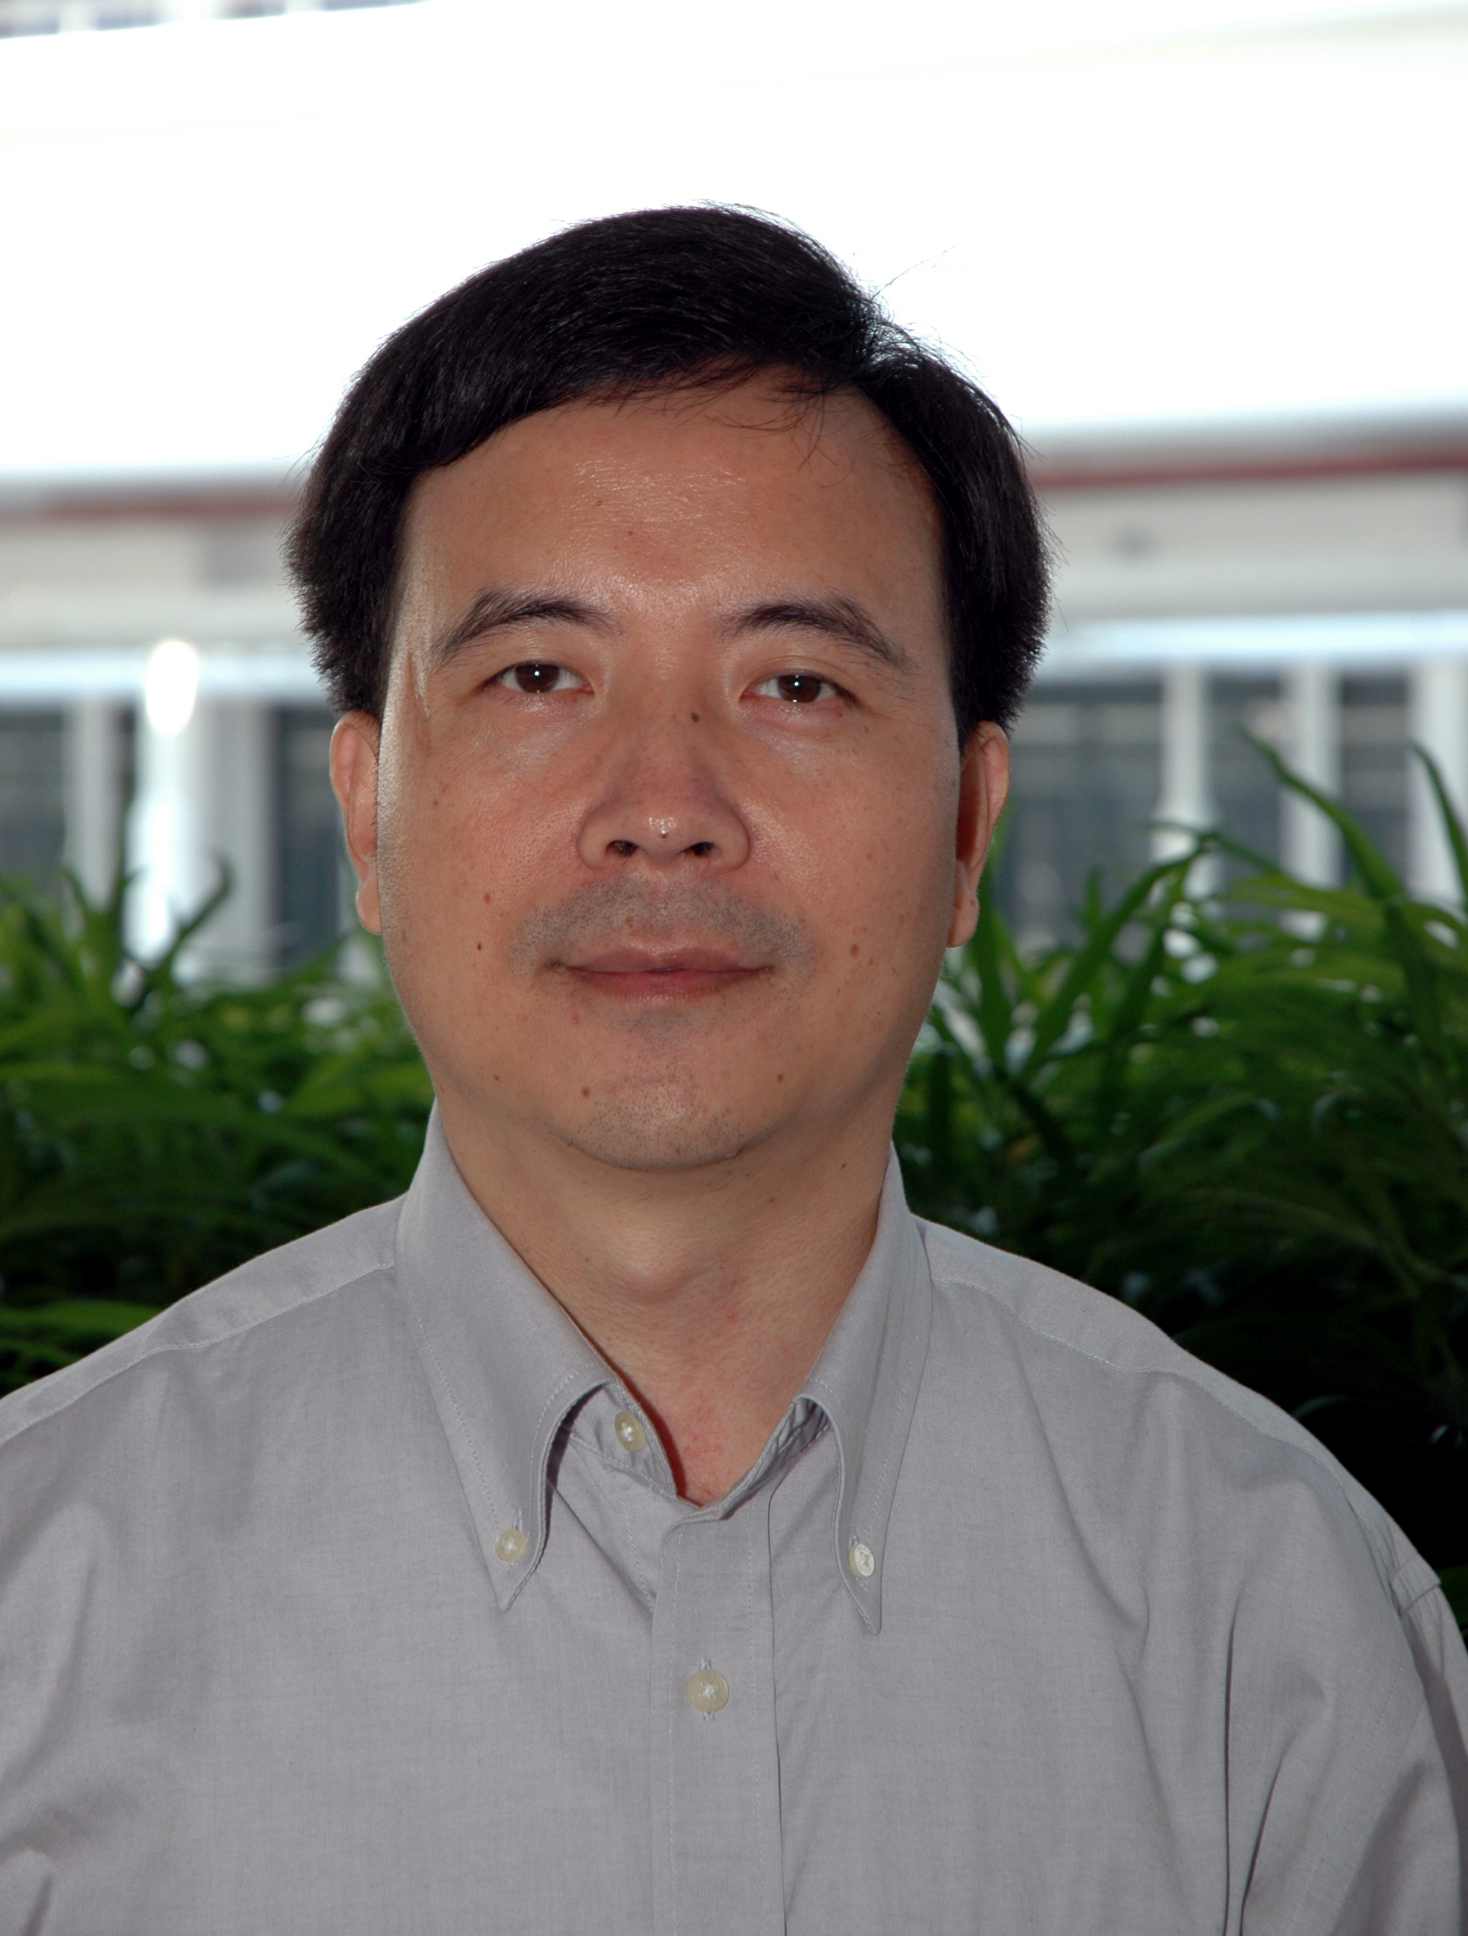
\includegraphics[width=1in,height=1.25in,clip,keepaspectratio]{photos/xie.jpg}}]{Lihua Xie}
	received the B.E. and M.E. degrees in electrical engineering from Nanjing University of Science and Technology in 1983 and 1986, respectively, and the Ph.D. degree in electrical engineering from the University of Newcastle, Australia, in 1992. Since 1992, he has been with the School of Electrical and Electronic Engineering, Nanyang Technological University, Singapore, where he is currently a professor and Director, Delta-NTU Corporate Laboratory for Cyber-Physical Systems. He served as the Head of Division of Control and Instrumentation from July 2011 to June 2014. He held teaching appointments in the Department of Automatic Control, Nanjing University of Science and Technology from 1986 to 1989. 
	
	Dr Xie's research interests include robust control and estimation, networked control systems, multi-agent networks, localization and unmanned systems. He is an Editor-in-Chief for Unmanned Systems and an Associate Editor for IEEE Transactions on Control of Network Systems. He has served as an editor of IET Book Series in Control and an Associate Editor of a number of journals including IEEE Transactions on Automatic Control, Automatica, IEEE Transactions on Control Systems Technology, and IEEE Transactions on Circuits and Systems-II. He is an elected member of Board of Governors, IEEE Control System Society (Jan 2016-Dec 2018). Dr. Xie is a Fellow of IEEE and Fellow of IFAC.
\end{IEEEbiography}


% You can push biographies down or up by placing
% a \vfill before or after them. The appropriate
% use of \vfill depends on what kind of text is
% on the last page and whether or not the columns
% are being equalized.

%\vfill

% Can be used to pull up biographies so that the bottom of the last one
% is flush with the other column.
%\enlargethispage{-5in}



% that's all folks
\end{document}


